\setcounter{section}{0}%更改chapter的计数器值
%\numberwithin{equation}{chapter}%公式计数器从属于节计数器
\numberwithin{equation}{section}%公式计数器从属于节计数器
\numberwithin{figure}{section}%图计数器从属于节计数器
\setcounter{chapter}{6}

%\chapter{\texorpdfstring{一圈振幅}{7 One-loop amplitudes}}
\chapter{一圈振幅}
在讨论几个相关曲面后,我们将集中于环面,首先是环面上的CFT,其次是散射振幅. 然后,我们推广至开弦和非定向弦理论. 最重要的议题是理解如何禁止短距离UV发散.

%\section{\texorpdfstring{Riemann面}{7.1 Riemann surfaces}}
\section{Riemann面}
有4种Euler为零的Riemann面.\\

\centerline{\Large 环面}
5.1节所讨论的环面 $T^{2}$是唯一 Euler为零的定向闭曲面. 我们将其描述成复平面,有度规 $d s^{2}=d w d \bar{w}$ 并有等价关系
\begin{equation}
	w \cong w+2 \pi \cong w+2 \pi \tau
\end{equation}
有两个模, $\tau=\tau_{1}+i \tau_{2}$的实部和虚部, 并有两个CKV,平移. 以实坐标 $w=\sigma^{1}+i \sigma^{2}$的形式
\begin{equation}
	\left(\sigma^{1}, \sigma^{2}\right) \cong\left(\sigma^{1}+2 \pi, \sigma^{2}\right) \cong\left(\sigma^{1}+2 \pi \tau_{1}, \sigma^{2}+2 \pi \tau_{2}\right)
\end{equation}
这使得我们可将环面视为底边周长 $2 \pi$ ,高$2 \pi \tau_{2}$ 的圆柱,但末端旋转了 $2 \pi \tau_{1}$ 然后粘在一起.\\
以坐标 $z=\exp (-i w)$, 等价关系 $w \cong w+2 \pi$ 是自动的,而 $w \cong w+2 \pi \tau$变成
\begin{equation}
	z \cong z \exp (-2 \pi i \tau)
\end{equation}
基本区域是圆环
\begin{equation}
	1 \leq|z| \leq \exp \left(2 \pi \tau_{2}\right)
\end{equation}
环面通过将外圆旋转 $2 \pi \tau_{1}$ 再与内圆粘合得到. 除非另有说明,我们将使用 $w$ 坐标.\\

\centerline{\Large The cylinder (annulus)}
圆柱$C_{2}$ 是
\begin{equation}
	0 \leq \operatorname{Re} w \leq \pi, \quad w \cong w+2 \pi i t
\end{equation}
即宽为 $\pi$ 长为 $2 \pi t$的带,但带的两端粘在一起. 只有一个模 $t$, 范围 $0<t<\infty $ . 不像环面,这里没有模群,长圆柱极限 $t \rightarrow 0$ 与长带极限 $t \rightarrow \infty$相当不同,只有一个CKV,平行于边界的平移. \\
圆柱可以从$\tau=i t$ 的环面中获得. 通过如下的对合等价
\begin{equation}
	w^{\prime}=-\bar{w}
\end{equation}
这是关于虚轴的反射. 线 $\sigma^{1}=0, \pi$ 被这一反射固定,因而变成边界. 另一坐标是周期等价
\begin{equation}
	\left(\sigma^{1}, 0\right) \cong\left(\sigma^{1}, 2 \pi t\right)
\end{equation}

\centerline{\Large Klein瓶}
Klein瓶 $K_{2}$ 可以视为复平面,但有等价
\begin{equation}
	w \cong w+2 \pi \cong-\bar{w}+2 \pi i t
\end{equation}
或者
\begin{equation}
	\left(\sigma^{1}, \sigma^{2}\right) \cong\left(\sigma^{1}+2 \pi, \sigma^{2}\right) \cong\left(-\sigma^{1}, \sigma^{2}+2 \pi t\right)
\end{equation}
这是周长$2 \pi$ ,高 $2 \pi t$的圆柱,但末端的宇称 $\Omega $反粘在一起.  单模 $t$ 取遍 $0<t<\infty$, 且没有模群.  $\sigma^{2}$ 方向的平移是唯一的CKV. Klein瓶可以从$\tau=2 i t$ 的环面获得,但要有等价关系
\begin{equation}
	w^{\prime}=-\bar{w}+2 \pi i t
\end{equation}
Klein瓶也可以视为有两个十字帽的球面.\\

\centerline{\Large Möbius带}
Möbius 带 $M_{2}$ 可以经由$\Omega$从带中获得
\begin{equation}
	0 \leq \operatorname{Re} w \leq \pi, \quad w \cong-\bar{w}+\pi+2 \pi i t
\end{equation}
模 $t$从$0<t<\infty$ ,CKV是 $\sigma^{2}$ 平移. 它可以从$\tau=2 i t$ 的环面通过两次对合等价获得
\begin{equation}
	w^{\prime}=-\bar{w} \quad \text { and } \quad w^{\prime}=w+\pi(2 i t+1)
\end{equation}
Möbius带可以视为一个有十字帽的圆盘.\\

\section{环面上的共形场论}%{7.2 CFT on the torus}

\centerline{\Large 标量关联子}
正如球面的情况,我们从Green函数 (6.2.7)出发,它满足[\footnotemark[1]{note}]
\begin{equation}
	\frac{2}{\alpha^{\prime}} \bar{\partial} \partial G^{\prime}\left(w, \bar{w} ; w^{\prime}, \bar{w}^{\prime}\right)=-2 \pi \delta^{2}\left(w-w^{\prime}\right)+\frac{1}{4 \pi \tau_{2}}
\end{equation}

\footnotetext[1]{note:从(6.2.8),\quad $g^{-1 / 2}=1 ,\quad \delta^{2}\left(\sigma_{1}-\sigma_{2}\right)=2 \delta^{2}\left(w-w^{\prime}\right)$
	$$
	\int d^{2} z x_{0}^{2}=1 \Rightarrow(2 \pi)^{2} \tau_{2} x_{0}^{2}=1 \Rightarrow x_{0}^{2}=\frac{1}{(2 \pi)^{2} \tau_{2}}
	$$
	(6.2.8)变成
	$$
	\begin{aligned}
	\frac{1}{2 \pi \alpha^{\prime}} \nabla^{2} G^{\prime} &=-2 \delta^{2}\left(w-w^{\prime}\right)+\frac{1}{4 \pi^{2} \tau_{2}} \\
	\frac{4 \bar{\partial} \partial G^{\prime}}{2 \alpha^{\prime}} &=-2 \lambda \delta^{2}\left(\omega-w^{\prime}\right)+\frac{1}{4 \pi \tau_{2}}
	\end{aligned}
	$$
	再利用$\nabla^{2}=4\bar{\partial} \partial$.\\
}


Green函数关于环面的两个方向都是周期的,并且除掉源项与背景荷项后,它应该是全纯函数与反全纯函数的和. 这些性质将它与 theta函数相联系. 我们猜测 
\begin{equation}
	G^{\prime}\left(w, \bar{w} ; w^{\prime}, \bar{w}^{\prime}\right) \sim-\frac{\alpha^{\prime}}{2} \ln \left|\vartheta_{1}\left(\frac{w-w^{\prime}}{2 \pi} \mid \tau\right)\right|^{2}
\end{equation}
当 $\vartheta_{1}$ 的变量趋于零时,它线性趋于零,给出了 $w \rightarrow w^{\prime} $的正确行为.  然而,由于准周期性(7.2.32b),它不是完全双周期的. 它在$w \rightarrow w+2 \pi \tau$下会改变 $-\alpha^{\prime}\left[\operatorname{Im}\left(w-w^{\prime}\right)+\pi \tau_{2}\right]$ . 另外背景电荷是缺失的,这两点都可以被轻松修正 :
\begin{equation}
	G^{\prime}\left(w, \bar{w} ; w^{\prime}, \bar{w}^{\prime}\right)=-\frac{\alpha^{\prime}}{2} \ln \left|\vartheta_{1}\left(\frac{w-w^{\prime}}{2 \pi} \mid \tau\right)\right|^{2}+\alpha^{\prime} \frac{\left[\operatorname{Im}\left(w-w^{\prime}\right)\right]^{2}}{4 \pi \tau_{2}}+k(\tau, \bar{\tau})
\end{equation}
函数$k(\tau, \bar{\tau})$ 通过 $\mathrm{X}_{0}$的正交性决定. 但同球面的情况一样,它由于时空动量守恒被丢掉了. 平行于之前的结果 (6.2.13) ,顶点算符的期望值
\begin{equation}
	\begin{aligned}
		\left\langle\prod_{i=1}^{n}:\right.&\left.e^{i k_{i} \cdot X\left(z_{i}, \bar{z}_{i}\right)}:\right\rangle_{T^{2}}=i C_{T^{2}}^{X}(\tau)(2 \pi)^{d} \delta^{d}\left(\sum_{i} k_{i}\right) \\
		& \times \prod_{i<j}\left|\frac{2 \pi}{\partial_{v} \vartheta_{1}(0 \mid \tau)} \vartheta_{1}\left(\frac{w_{i j}}{2 \pi} \mid \tau\right) \exp \left[-\frac{\left(\operatorname{Im} w_{i j}\right)^{2}}{4 \pi \tau_{2}}\right]\right|^{\alpha^{\prime} k_{i} \cdot k_{j}}
	\end{aligned}
\end{equation}
因子 $2 \pi / \partial_{v} \vartheta_{1}$来自于重整化自收缩.\\

\centerline{\Large 标量配分函数}
球面的总归一化被吸收进弦的耦合常数中,但我们不能对环面做相同的事,这主要是这里存在一个非平庸的$\tau$相关性. 事实上,我们将从没有顶点算符的振幅中看到一大堆物理. 考察没有顶点算符的路径积分 $\langle 1\rangle_{T^{2}(\tau)} \equiv Z(\tau) $,我们可以将模 $\tau$ 的环面视为一个圆上的场论,它演化了 Euclidean时间 $2 \pi \tau_{2}$,沿$\sigma^{1}$ 方向平移了 $2 \pi \tau_{1}$, 然后将两端等同. 以算符的语言这给出了迹[\footnotemark[2]{note}]
\begin{equation}
	\begin{aligned}
		Z(\tau) &=\operatorname{Tr}\left[\exp \left(2 \pi i \tau_{1} P-2 \pi \tau_{2} H\right)\right] \\
		&=(q \bar{q})^{-d / 24} \operatorname{Tr}\left(q^{L_{0}} \bar{q}^{\tilde{L}_{0}}\right)
	\end{aligned}
\end{equation}

\footnotetext[2]{note:$$
	\begin{aligned}
	&e^{2 \pi i \tau_{1}\left(L_{0}-\tilde{L}_{0}\right)}-2 \pi \tau_{2}\left(L_{0}+\widetilde{L}_{0}-d/12\right)\\
	=&e^{2 \pi i\left(\tau_{1}+i \tau_{2}\right) L_{0}} e^{-2 \pi i\left(\tau_{1}-i \tau_{2}\right) \tilde{L}_{0}}(q \bar{q})^{-d / 24}\\
	=&q^{L_0}\bar{q}^{\tilde{L}_0}(q \bar{q})^{-d / 24}
	\end{aligned}
	$$
$$
q \bar{q}=e^{2 \pi i\left(\tau_{1}+i \tau_{2}\right)} e^{-2 \pi i\left(\tau_{1}-i \tau_{2}\right)} =e^{-4 \pi \tau_{2}}
$$}



这里 $q=\exp (2 \pi i \tau)$, 动量 $P=L_{0}-\tilde{L}_{0}$ 生成 $\sigma^{1}$方向的平移, Hamiltonian $H=L_{0}+\tilde{L}_{0}-\frac{1}{24}(c+\tilde{c})$ 生成 $\sigma^{2}$ 方向的平移 . 这种迹被赋予了Hamiltonian和其他守恒量的指数,就像统计力学那样,被称为配分函数.\\

这个迹可以分成对占有数 $N_{\mu n}$ 和$\tilde{N}_{\mu n}$ 的求和以及对动量$k^{\mu}$的积分.  $Z(\tau)$ 变成[\footnotemark[3]{note}]
\begin{equation}
	V_{d}(q \bar{q})^{-d / 24} \int \frac{d^{d} k}{(2 \pi)^{d}} \exp \left(-\pi \tau_{2} \alpha^{\prime} k^{2}\right) \prod_{\mu, n} \sum_{N_{\mu n}, \tilde{N}_{\mu n}=0}^{\infty} q^{n N_{\mu n}} \bar{q}^{n \tilde{N}_{\mu n}}
\end{equation}

\footnotetext[3]{note:$$L_{0}=\frac{\alpha^{\prime} p^{2}}{4}+\sum a_{-n} a_{n}$$
$$
\begin{aligned}
q^{L_0} \bar{q}^{L_0} &=e^{2 \pi(-\tau_{2}+i \tau_{1})\frac{\alpha^{\prime} p^2} {4}}  e^{2 \pi(-\tau_{2}-i c_{1}) \frac{\alpha^{\prime} p^{2}}{4}} \\
&=e^{-4 \pi \tau_{2} \frac{\alpha^{\prime} p^{2}}{4}}=e^{-\pi\tau_{2} \alpha^{\prime} p^{2}}
\end{aligned}
$$}

时空体积因子$V_{d}$来自于动量的连续归一化, $\sum_{k}$ becoming $V_{d}(2 \pi)^{-d} \int d^{d} k$. 求和是几何级数
\begin{equation}
	\sum_{N=0}^{\infty} q^{n N}=\left(1-q^{n}\right)^{-1}
\end{equation}
由此获得
\begin{equation}
	Z(\tau)=i V_{d} Z_{X}(\tau)^{d}
\end{equation}
其中
\begin{equation}
	Z_{X}(\tau)=\left(4 \pi^{2} \alpha^{\prime} \tau_{2}\right)^{-1 / 2}|\eta(\tau)|^{-2}
\end{equation}
这里
\begin{equation}
	\eta(\tau)=q^{1 / 24} \prod_{n=1}^{\infty}\left(1-q^{n}\right)
\end{equation}
是Dedekind eta函数. 这里的 $i$来自于旋转 $k^{0} \rightarrow i k^{d}$ .另外,之前的 $C_{T^{2}}^{X}(\tau)=Z_{X}(\tau)^{d}$.\\
 (7.2.8) is 在 $\tau \rightarrow \tau+1$下显然不变.  $Z_{X}$在 $\tau \rightarrow-1 / \tau$ 党的不变性由 (7.2.44)$\eta(-1 / \tau)=(-i \tau)^{1 / 2} \eta(\tau)$给出. 这生成了整个模群. 类似地,含有顶点算符的期望值也是模协变的. \\
这个计算可以利用全纯性完成. 思想是得到关于$\tau$的微分方程. 考察模为 $\tau$的环面,并对度规做一个小改变 $\delta g_{w w}=\epsilon^{*}$. 新度规是
\begin{equation}
	\begin{aligned}
		d s^{2} &=d w d \bar{w}+\epsilon^{*} d w^{2}+\epsilon d \bar{w}^{2} \\
		&=\left(1+\epsilon^{*}+\epsilon\right) d[w+\epsilon(\bar{w}-w)] d\left[\bar{w}+\epsilon^{*}(w-\bar{w})\right]+O\left(\epsilon^{2}\right)
	\end{aligned}
\end{equation}
即,这一度规Weyl等价于$d w^{\prime} d \bar{w}^{\prime}$,其中 $w^{\prime}=w+\epsilon(\bar{w}-w)$. 它有周期性
\begin{equation}
	w^{\prime} \cong w^{\prime}+2 \pi \cong w^{\prime}+2 \pi\left(\tau-2 i \tau_{2} \epsilon\right)
\end{equation}
度规的改变因而等价于模的改变
\begin{equation}
	\delta \tau=-2 i \tau_{2} \epsilon
\end{equation}
在改变度规后,路径积分的改变为
\begin{equation}
	\begin{aligned}
		\delta Z(\tau) &=-\frac{1}{2 \pi} \int d^{2} w\left[\delta g_{\bar{w} \bar{w}}\left\langle T_{w w}(w)\right\rangle+\delta g_{w w}\left\langle T_{\bar{w} \bar{w}}(\bar{w})\right\rangle\right] \\
		&=-2 \pi i\left[\delta \tau\left\langle T_{w w}(0)\right\rangle-\delta \bar{\tau}\left\langle T_{\bar{w} \bar{w}}(0)\right\rangle\right]
	\end{aligned}
\end{equation}

在第二行,我们用平移不变性做了积分. 为得到能动张量期望值,我们用OPE
\begin{equation}
\partial_{w} X^{\mu}(w) \partial_{w} X_{\mu}(0)=-\frac{\alpha^{\prime} d}{2 w^{2}}-\alpha^{\prime} T_{w w}(0)+O(w)
\end{equation}
现在
\begin{equation}
\begin{aligned}
Z(\tau)^{-1}\left\langle\partial_{w} X^{\mu}(w) \partial_{w} X_{\mu}(0)\right\rangle &=\left.d \partial_{w} \partial_{w^{\prime}} G^{\prime}\left(w, \bar{w} ; w^{\prime}, \bar{w}^{\prime}\right)\right|_{w^{\prime}=0} \\
&=\frac{\alpha^{\prime} d}{2} \frac{\vartheta_{1} \partial_{w}^{2} \vartheta_{1}-\partial_{w} \vartheta_{1} \partial_{w} \vartheta_{1}}{\vartheta_{1}^{2}}+\frac{\alpha^{\prime} d}{8 \pi \tau_{2}}
\end{aligned}
\end{equation}
其中所有theta函数的变量是$(w / 2 \pi, \tau)$. 它确实在 $w=0 $ 有双极点. 小心地将分子、分母展开到 $w^{2}$、 $w^{0}$ 阶是
\begin{equation}
\frac{\alpha^{\prime} d}{6} \frac{\partial_{w}^{3} \vartheta_{1}}{\partial_{w} \vartheta_{1}}+\frac{\alpha^{\prime} d}{8 \pi \tau_{2}}
\end{equation}
那么OPE (7.2.15) 给出
\begin{equation}
\left\langle T_{w w}(0)\right\rangle=\left(-\frac{d}{6} \frac{\partial_{w}^{3} \vartheta_{1}(0 \mid \tau)}{\partial_{w} \vartheta_{1}(0 \mid \tau)}-\frac{d}{8 \pi \tau_{2}}\right) Z(\tau)
\end{equation}
变分 (7.2.14) 给出微分方程
\begin{equation}
\partial_{\tau} \ln Z(\tau)=\frac{\pi i d}{3} \frac{\partial_{w}^{3} \vartheta_{1}(0 \mid \tau)}{\partial_{w} \vartheta_{1}(0 \mid \tau)}+\frac{i d}{4 \tau_{2}}
\end{equation}
为了更进一步,利用
\begin{equation}
\partial_{w}^{2} \vartheta_{1}\left(\frac{w}{2 \pi} \mid \tau\right)=\frac{i}{\pi} \partial_{\tau} \vartheta_{1}\left(\frac{w}{2 \pi} \mid \tau\right)
\end{equation}
将(7.2.19) 重写为
\begin{equation}
\partial_{\tau} \ln Z(\tau)=-\frac{d}{3} \partial_{\tau} \ln \partial_{w} \vartheta_{1}(0 \mid \tau)+\frac{i d}{4 \tau_{2}}
\end{equation}
与共轭方程一起,这给出
\begin{equation}
Z(\tau)=\left|\partial_{w} \vartheta_{1}(0 \mid \tau)\right|^{-2 d / 3} \tau_{2}^{-d / 2}
\end{equation}
会相差一个数值系数,要用其他方法决定. 利用 (7.2.43), ,可以看到它与 (7.2.8)一致.\\

\centerline{\Large  bc CFT}
对于鬼场CFT,配分函数也可由态的迹决定. 在左边和右边均有两组产生算符 $b_{-n}$ 和 $c_{-n}$ ,但它们是反对易的. 所以占有数只能是0或1. 因此在模n的振子给出 $\left(1+q^{n}\right) $ . 另外存在4个基态,这给出
\begin{equation}
\begin{aligned}
\operatorname{Tr}\left[\exp \left(2 \pi i \tau_{1} P-2 \pi \tau_{2} H\right)\right] &=(q \bar{q})^{13 / 12} \operatorname{Tr}\left(q^{L_{0}} \bar{q}^{\tilde{L}_{0}}\right) \\
&=4(q \bar{q})^{1 / 12} \prod_{n=1}^{\infty}\left|1+q^{n}\right|^{4}
\end{aligned}
\end{equation}
然而,对于反对易场,这个迹对应于在时间方向上有反周期边界的路径积分. 为了计算Faddeev-Popov 行列式,鬼场必须与原始坐标变换的周期性相同,而这是周期的. 因此我们需要
\begin{equation}
\begin{aligned}
Z(\tau) &=\operatorname{Tr}\left[(-1)^{F} \exp \left(2 \pi i \tau_{1} P-2 \pi \tau_{2} H\right)\right] \\
&=0
\end{aligned}
\end{equation}
其中$(-1)^{F}$ 与所有鬼场反对易. 该迹为零是因为 $|\downarrow \downarrow\rangle$ 和 $|\uparrow \uparrow\rangle$ 的鬼数与 $|\uparrow \downarrow\rangle$ 和 $|\downarrow \uparrow\rangle $的鬼数在模掉之后相反. 从路径积分观点看, $Z(\tau)$ 为零是由于模与CKV的鬼零模. 它们必须要浸入道合适的插入,最简单的不为零的振幅是
\begin{equation}
\left\langle c\left(w_{1}\right) b\left(w_{2}\right) \tilde{c}\left(\bar{w}_{3}\right) \tilde{b}\left(\bar{w}_{4}\right)\right\rangle
\end{equation}
在算符计算中,我们将每一场写成它的模展开. 仅有$n=0$的项有贡献. 那么$(7.2 .25)$ 变成
\begin{equation}
\operatorname{Tr}\left[(-1)^{F} c_{0} b_{0} \tilde{c}_{0} \tilde{b}_{0} \exp \left(2 \pi i \tau_{1} P-2 \pi \tau_{2} H\right)\right]
\end{equation}
算符 $c_{0} b_{0} \tilde{c}_{0} \tilde{b}_{0}$ 投影到基态$|\uparrow \uparrow\rangle$, 所以结果是
\begin{equation}
(q \bar{q})^{1 / 12} \prod_{n=1}^{\infty}\left|1-q^{n}\right|^{4}=|\eta(\tau)|^{4}
\end{equation}
注意无穷乘积中的符号改变,来自迹中的 $(-1)^{F}$. 由于环面上的CKV与二次微分是常数,所以 (7.2.27)与鬼场的位置无关.\\

\centerline{\Large 一般CFT}
对于一般的CFT
\begin{equation}
Z(\tau)=\sum_{i} q^{h_{i}-c / 24} \bar{q}^{\tilde{h}_{i}-\tilde{c} / 24}(-1)^{F_{i}}
\end{equation}
其中i取遍CFT的所有态,而 $F_{i}$ 是世界面Fermion数. 在 $\tau \rightarrow \tau+1$ 下不变要求 $h_{i}-\tilde{h}_{i}-\frac{1}{24}(c-\tilde{c})$ 为整数. 观察单位算符,这要求$c-\tilde{c}$是24的倍数. 那么对于一般的算符,就要求自旋为整数
\begin{equation}
h_{i}-\tilde{h}_{i} \in \mathbf{Z}
\end{equation}
顺带地, $c-\tilde{c}$ 不是24倍数的CFT也必然是有趣的. 它们无法单独是模不变的,但有了合适的投影,它们可以被整合进一个模不变的理论.\\
$\tau \rightarrow-1 / \tau$ 的不变性,这给频谱附加了进一步的限制. 考察 $\tau=i \ell$的配分函数,并令 $\ell \rightarrow 0 $ ,收敛因子 $q=\exp (-2 \pi \ell)$ 趋于1. 所以配分函数由最高权重态的密度决定. 利用模不变性这等于 $\tau=i / \ell $的配分函数,而后者$q=\exp (-2 \pi / \ell)$ 趋于0. 所以最低权重态主导求和,这是单位态,并有$L_{0}=\tilde{L}_{0}=0$, 给出
\begin{equation}
Z(i \ell) \stackrel{l \rightarrow 0}{\approx} \exp \left[\frac{\pi(c+\tilde{c})}{12 \ell}\right]
\end{equation}
最高权重态的密度因此由中心荷决定. 这生成了自由玻色子的结果,其中 $c=\tilde{c}=d$计数了自由玻色子数目.\\

\centerline{\Large Theta函数}
基本theta函数是
\begin{equation}
	\vartheta(v, \tau)=\sum_{n=-\infty}^{\infty} \exp \left(\pi i n^{2} \tau+2 \pi i n v\right)
\end{equation}
它有周期性
\begin{subequations}
\begin{equation}
\vartheta(v+1, \tau)=\vartheta(v, \tau) 
\end{equation}
\begin{equation}
\vartheta(v+\tau, \tau)=\exp (-\pi i \tau-2 \pi i v) \vartheta(v, \tau)
\end{equation}
\end{subequations}
在模变换下
\begin{subequations}
\begin{equation}
\vartheta(v, \tau+1) =\vartheta(v+1 / 2, \tau)
\end{equation}
\begin{equation}
\vartheta(v / \tau,-1 / \tau) =(-i \tau)^{1 / 2} \exp \left(\pi i v^{2} / \tau\right) \vartheta(v, \tau)
\end{equation}
\end{subequations}
除去周期性(7.2.32), theta函数只有一个零点 $v=\frac{1}{2}(1+\tau) $ . 它同时也可写成无穷乘积
\begin{equation}
	\vartheta(v, \tau)=\prod_{m=1}^{\infty}\left(1-q^{m}\right)\left(1+z q^{m-1 / 2}\right)\left(1+z^{-1} q^{m-1 / 2}\right)
\end{equation}
其中
\begin{equation}
	q=\exp (2 \pi i \tau), \quad z=\exp (2 \pi i v)
\end{equation}
我们通常需要theta函数在 $q \rightarrow 0$ 或 $q \rightarrow 1$的渐近行为.  $q \rightarrow 0$ 可从无穷乘积或无限求和中立即读出, $q \rightarrow 1$ 的行为并不显然,它可以从 $\tau \rightarrow-1 / \tau$ 的模变换中获得,这通过$q \rightarrow \exp \left(4 \pi^{2} / \ln q\right)$将将两个极限关联起来.\\
定义有特征的theta函数通常是有用的
\begin{equation}
	\begin{aligned}
		\vartheta\left[\begin{array}{c}
			a \\
			b
		\end{array}\right](v, \tau) &=\exp \left[\pi i a^{2} \tau+2 \pi i a(v+b)\right] \vartheta(v+a \tau+b, \tau) \\
		&=\sum_{n=-\infty}^{\infty} \exp \left[\pi i(n+a)^{2} \tau+2 \pi i(n+a)(v+b)\right]
	\end{aligned}
\end{equation}
其他常用记法
\begin{subequations}
\begin{equation}
\vartheta_{00}(v, \tau)=\vartheta_{3}(v \mid \tau)=\vartheta\left[\begin{array}{l}
0 \\
0
\end{array}\right](v, \tau)=\sum_{n=-\infty}^{\infty} q^{n^{2} / 2} z^{n} 
\end{equation}
\begin{equation}
\vartheta_{01}(v, \tau)=\vartheta_{4}(v \mid \tau)=\vartheta\left[\begin{array}{c}
0 \\
1 / 2
\end{array}\right](v, \tau)=\sum_{n=-\infty}^{\infty}(-1)^{n} q^{n^{2} / 2} z^{n}
\end{equation}
\begin{equation}
\vartheta_{10}(v, \tau)=\vartheta_{2}(v \mid \tau) =\vartheta\left[\begin{array}{c}
1 / 2 \\
0
\end{array}\right](v, \tau)=\sum_{n=-\infty}^{\infty} q^{(n-1 / 2)^{2} / 2} z^{n-1 / 2} 
\end{equation}
\begin{equation}
\vartheta_{11}(v, \tau)=-\vartheta_{1}(v \mid \tau) =\vartheta\left[\begin{array}{l}
1 / 2 \\
1 / 2
\end{array}\right](v, \tau) =-i \sum_{n=-\infty}^{\infty}(-1)^{n} q^{(n-1 / 2)^{2} / 2} z^{n-1 / 2}
\end{equation}
\end{subequations}
乘积表示:
\begin{subequations}
\begin{equation}
\vartheta_{00}(v, \tau)=\prod_{m=1}^{\infty}\left(1-q^{m}\right)\left(1+z q^{m-1 / 2}\right)\left(1+z^{-1} q^{m-1 / 2}\right) 
\end{equation}
\begin{equation}
\vartheta_{01}(v, \tau)=\prod_{m=1}^{\infty}\left(1-q^{m}\right)\left(1-z q^{m-1 / 2}\right)\left(1-z^{-1} q^{m-1 / 2}\right)
\end{equation}
\begin{equation}
\vartheta_{10}(v, \tau)=2 \exp (\pi i \tau / 4) \cos \pi v \prod_{m=1}^{\infty}\left(1-q^{m}\right)\left(1+z q^{m}\right)\left(1+z^{-1} q^{m}\right) 
\end{equation}
\begin{equation}
\vartheta_{11}(v, \tau)=-2 \exp (\pi i \tau / 4) \sin \pi v \prod_{m=1}^{\infty}\left(1-q^{m}\right)\left(1-z q^{m}\right)\left(1-z^{-1} q^{m}\right) 
\end{equation}	
\end{subequations}
模变换
\begin{subequations}
\begin{equation}
\vartheta_{00}(v, \tau+1)=\vartheta_{01}(v, \tau) 
\end{equation}
\begin{equation}
\vartheta_{01}(v, \tau+1)=\vartheta_{00}(v, \tau) 
\end{equation}
\begin{equation}
\vartheta_{10}(v, \tau+1)=\exp (\pi i / 4) \vartheta_{10}(v, \tau)
\end{equation}
\begin{equation}
\vartheta_{11}(v, \tau+1)=\exp (\pi i / 4) \vartheta_{11}(v, \tau)
\end{equation}
\end{subequations}
以及
\begin{subequations}
	\begin{equation}
		\vartheta_{00}(v / \tau,-1 / \tau) =(-i \tau)^{1 / 2} \exp \left(\pi i v^{2} / \tau\right) \vartheta_{00}(v, \tau)
\end{equation}
\begin{equation}		
		\vartheta_{01}(v / \tau,-1 / \tau) =(-i \tau)^{1 / 2} \exp \left(\pi i v^{2} / \tau\right) \vartheta_{10}(v, \tau)
\end{equation}
\begin{equation}		
		\vartheta_{10}(v / \tau,-1 / \tau) =(-i \tau)^{1 / 2} \exp \left(\pi i v^{2} / \tau\right) \vartheta_{01}(v, \tau) 
\end{equation}
\begin{equation}		
		\vartheta_{11}(v / \tau,-1 / \tau) =-i(-i \tau)^{1 / 2} \exp \left(\pi i v^{2} / \tau\right) \vartheta_{11}(v, \tau)
\end{equation}
\end{subequations}
在超弦中我们将会更加频繁地遇到这些函数. theta函数满足 Jacobi的 'abstruse等式',即Riemann等式的一种特殊情况
\begin{equation}
	\vartheta_{00}^{4}(0, \tau)-\vartheta_{01}^{4}(0, \tau)-\vartheta_{10}^{4}(0, \tau)=0
\end{equation}
同时注意到
\begin{equation}
	\vartheta_{11}(0, \tau)=0
\end{equation}
最终,Dedekind eta函数是
\begin{equation}
	\eta(\tau)=q^{1 / 24} \prod_{m=1}^{\infty}\left(1-q^{m}\right)=\left[\frac{\partial_{v} \vartheta_{11}(0, \tau)}{-2 \pi}\right]^{1 / 3}
\end{equation}
模变换
\begin{subequations}
\begin{equation}
\eta(\tau+1)=\exp (i \pi / 12) \eta(\tau) 
\end{equation}
\begin{equation}
\eta(-1 / \tau)=(-i \tau)^{1 / 2} \eta(\tau)
\end{equation}
\end{subequations}

\section{环面振幅}%{7.3 The torus amplitude}
我们现在对环面应用一般结果(5.3.9) ,将弦的散射振幅表述为有鬼场和顶点算符插入的积分. 两个CKV要求一个顶点算符被固定,所以
\begin{equation}
	\begin{aligned}
		&S_{T^{2}}(1 ; 2 ; \ldots ; n) \\
		&\quad=\frac{1}{2} \int_{F_{0}} d \tau d \bar{\tau}\left\langle B \tilde{B} \tilde{c} c \mathscr{V}_{1}\left(w_{1}, \bar{w}_{1}\right) \prod_{i=2}^{n} \int d w_{i} d \bar{w}_{i} \mathscr{V}_{i}\left(w_{i}, \bar{w}_{i}\right)\right\rangle_{T^{2}}
	\end{aligned}
\end{equation}
基本区域 $F_{0}$ 和5.1节讨论的一样, $\frac{1}{2}$来自于 $w \rightarrow-w$. 如同复变量场,$d \tau d \bar{\tau}=2 d \tau_{1} d \tau_{2}$ 其中 $\tau=\tau_{1}+i \tau_{2}$.  $d \tau$ 的鬼场插入是
\begin{equation}
	\begin{aligned}
		B=\frac{1}{4 \pi}\left(b, \partial_{\tau} g\right) &=\frac{1}{2 \pi} \int d^{2} w b_{w w}(w) \partial_{\tau} g_{\bar{w} \bar{w}} \\
		&=\frac{i}{4 \pi \tau_{2}} \int d^{2} w b_{w w}(w) \\
		& \rightarrow 2 \pi i b_{w w}(0)
	\end{aligned}
\end{equation}
我们使用了 (7.2.13) . 最后一行我们利用了鬼场路径积分 $(7.2 .27)$ 与位置无关. \\
CKG由环面的平移构成. 既然这个群体积有限,我们不需要固定它,我们可以重写振幅使得所有顶点算符都被积掉而CKG的体积被除掉. CKV是常数,所以(7.3.1)中的期望值独立于c的位置:我们可以让c远离$w_{1}$, 将它们放在某个固定位置上. 对于顶点算符,平移不变性暗示了振幅在 $w_{i} \rightarrow w_{i}+w$下不变. 对这一平移做平均
\begin{equation}
	\int \frac{d w d \bar{w}}{2(2 \pi)^{2} \tau_{2}}
\end{equation}
分母是环面的面积,这是CKG的体积.利用 (7.3.2) 和(7.3.3), 振幅变成
\begin{equation}
	\begin{aligned}
		&S_{T^{2}}(1 ; 2 ; \ldots ; n) \\
		&\quad=\int_{F_{0}} \frac{d \tau d \bar{\tau}}{4 \tau_{2}}\left\langle b(0) \tilde{b}(0) \tilde{c}(0) c(0) \prod_{i=1}^{n} \int d w_{i} d \bar{w}_{i} \mathscr{V}_{i}\left(w_{i}, \bar{w}_{i}\right)\right\rangle_{T^{2}}
	\end{aligned}
\end{equation}
同理现在所有顶点算符地位相同.\\

\fbox{\noindent\centering\parbox{0.9\textwidth}{因子来源:$$
		\begin{array}{*{20}c}
		{\frac{1}{2}} &  \times  & {\frac{1}{2}\frac{1}{{(2\pi )^2 \tau _2 }}} &  \times  & {(2\pi )^2 } &  =  & {\frac{1}{{4\tau _2 }}}  \\
		\uparrow  & {} &  \uparrow  & {} &  \uparrow  & {} & {}  \\
		{(7.3.1)} & {} & {(7.3.1)} & {} & {(7.3.1)} & {} & {}  \\
		\end{array}
		$$}}\\

不用固定顶点算符的中间步骤, (7.3.4)也可直接导出,甚至没有顶点算符,它也是成立的,
\begin{equation}
	Z_{T^{2}}=\int_{F_{0}} \frac{d \tau d \bar{\tau}}{4 \tau_{2}}\langle b(0) \tilde{b}(0) \tilde{c}(0) c(0)\rangle_{T^{2}}
\end{equation}
这一真空振幅相当有趣,将是我们研究的主要目标. 它不仅揭示了弦论的紫外行为与场论的紫外行为不同,它自身也有重要的物理意义.\\
对于26个平坦时空维,物质场和鬼场的路径积分 (7.3.5)已经在上一节计算过了,结果是
\begin{equation}
	Z_{T^{2}}=i V_{26} \int_{F_{0}} \frac{d \tau d \bar{\tau}}{4 \tau_{2}}\left(4 \pi^{2} \alpha^{\prime} \tau_{2}\right)^{-13}|\eta(\tau)|^{-48}
\end{equation}

\fbox{\noindent\centering\parbox{0.9\textwidth}{根据$\left[Z_{X}(\tau)\right]^{26}=\left(4 \pi^{2} \alpha^{\prime} C_{2}\right)^{-13}|\eta(\tau)|^{-52}$;
		根据(7.2.27),$\langle c b \tilde{c} \tilde{b}\rangle=|\eta(\tau)|^{4}$}}\\

这一振幅有重要性质:模不变. 根据(7.2.44), $\tau_{2}|\eta(\tau)|^{4}$ 是模不变的,也很容易验证
\begin{equation}
	\frac{d \tau d \bar{\tau}}{\tau_{2}^{2}}
\end{equation}
也是模不变的.\\

\fbox{\noindent\centering\parbox{0.9\textwidth}{$$
		\tau \rightarrow \tau+1 \rightarrow\left\{\begin{array}{l}
		\tau_{1} \rightarrow \tau_{1}+1 \\
		\tau_{2} \rightarrow \tau_{2}
		\end{array}\right.
		,\quad
	\tau \rightarrow-1 / \tau \rightarrow\left\{\begin{aligned}
	\tau_{1} & \rightarrow \frac{-\tau_{1}}{\tau_{1}^{2}+\tau_{2}^{2}} \\
	\tau_{2} & \rightarrow \frac{\tau_{2}}{\tau_{1}^{2}+\tau_{2}^{2}}
	\end{aligned}\right.
	$$
$$
\tau_{2}|\eta(\tau)|^{4} \rightarrow\frac{\tau_2}{|\tau|^2}|\eta(-1/\tau)|^4=\tau_2|\eta(\tau)|^4
$$
$$
\frac{d\tau d \bar{\tau}}{\tau_{2}^{2}}\rightarrow\frac{-\frac{1}{\tau^{2}}\left(-\frac{1}{\tau^{2}}\right) d \tau d\bar{\tau}}{\tau_{2}^{2} /|\tau|^{2}}=\frac{|\tau|^{2} d \tau d \bar{\tau}}{\tau_{2}^{2} /|\tau|^{2}}=\frac{d\tau d \bar{\tau}}{\tau_{2}^{2}}?
$$}}\\

注意到,指数-48来自24个左移振子和24个右移振子. 鬼的贡献抵消了两组振子,仅留下横向模的贡献. 通过给期望值  (7.2.4) 引入顶点算符并对位置积分,就给出了n快子的振幅. \\
对于一般的CFT,环面上的路径积分表述为 (7.2.28)中的迹. 只要存在 $d \geq 2$ 个非紧致平坦维,鬼场仍会抵消两组玻色算符,而真空振幅
\begin{subequations}
\begin{equation}
Z_{T^{2}} =V_{d} \int_{F_{0}} \frac{d \tau d \bar{\tau}}{4 \tau_{2}} \int \frac{d^{d} k}{(2 \pi)^{d}} \exp \left(-\pi \tau_{2} \alpha^{\prime} k^{2}\right) \sum_{i \in \mathscr{H}^{\perp}} q^{h_{i}-1} \bar{q}^{\tilde{h}_{i}-1} 
\end{equation}
\begin{equation}
=i V_{d} \int_{F_{0}} \frac{d \tau d \bar{\tau}}{4 \tau_{2}}\left(4 \pi^{2} \alpha^{\prime} \tau_{2}\right)^{-d / 2} \sum_{i \in \mathscr{H}^{\perp}} q^{h_{i}-1} \bar{q}^{\tilde{h}_{i}-1}
\end{equation}		
\end{subequations}
这里$\mathscr{H}^{\perp}$ 是去掉鬼、 $\mu=0,1$振子以及非紧致动量的闭弦Hilbert. 为了理解这些振幅的物理,与场论中的相应量进行比较将是有用的. 对所有拓扑为圆的路径求和,这由
\begin{equation}
	\begin{aligned}
		Z_{S_{1}}\left(m^{2}\right) &=V_{d} \int \frac{d^{d} k}{(2 \pi)^{d}} \int_{0}^{\infty} \frac{d l}{2 l} \exp \left[-\left(k^{2}+m^{2}\right) l / 2\right] \\
		&=i V_{d} \int_{0}^{\infty} \frac{d l}{2 l}(2 \pi l)^{-d / 2} \exp \left(-m^{2} l / 2\right)
	\end{aligned}
\end{equation}
给定. 这可以通过规范固定点粒子路径积分导出. 结果是直观的:$l$是圆的模, $\frac{1}{2}\left(k^{2}+m^{2}\right)$ 是世界线 Hamiltonian, $2 l$ 移去了来自平移的重复计数,以及反转世界线坐标的重复计数.\\
我们现在采用点粒子的结果,它所针对的粒子质量为 $m^{2}$, 并对弦的频谱求和. 正如第4章说过的,物理谱与 $\mathscr{H}^{\perp}$一一对应,其中质量与横向权重的关系
\begin{equation}
	m^{2}=\frac{2}{\alpha^{\prime}}(h+\tilde{h}-2)
\end{equation}
并有约束 $h=\tilde{h} $. 可将这一约束写成积分形式
\begin{equation}
	\delta_{h, \tilde{h}}=\int_{-\pi}^{\pi} \frac{d \theta}{2 \pi} \exp [i(h-\tilde{h}) \theta]
\end{equation}
在上式中,我们假定$h-\tilde{h}$是整数.这在26个平坦维下是正确的,正如上一节讨论的. 一般而言,模不变性是重要的. 那么
\begin{equation}
	\begin{aligned}
		\sum_{i \in \mathscr{H} \perp} Z_{S_{1}}\left(m_{i}^{2}\right)=i V_{d} \int_{0}^{\infty} & \frac{d l}{2 l} \int_{-\pi}^{\pi} \frac{d \theta}{2 \pi}(2 \pi l)^{-d / 2} \\
		& \times \sum_{i \in \mathscr{H}^{\perp}} \exp \left[-\left(h_{i}+\tilde{h}_{i}-2\right) l / \alpha^{\prime}+i\left(h_{i}-\tilde{h}_{i}\right) \theta\right] \\
		=& i V_{d} \int_{R} \frac{d \tau d \bar{\tau}}{4 \tau_{2}}\left(4 \pi^{2} \alpha^{\prime} \tau_{2}\right)^{-d / 2} \sum_{i \in \mathscr{H} \perp} q^{h_{i}-1} \bar{q}^{\tilde{h}_{i}-1}
	\end{aligned}
\end{equation}
其中 $\theta+i l / \alpha^{\prime}=2 \pi \tau$. 积分区域 $R$ :
\begin{equation}
	R: \quad \tau_{2}>0, \quad\left|\tau_{1}\right|<\frac{1}{2}
\end{equation}
我们现在来解释这一结果. 单个点粒子振幅 (7.3.9)在$l \rightarrow 0$发散. 这是通常的量子场论UV发散. 像(7.3.12)那样仅对弦频谱求和只会使情况更糟. 这时弦的所有贡献为同一符号. 然而,比较 (7.3.12) 与实际的弦振幅(7.3.8),它们非常相似但有一显著差异. 积分区域不同:在弦中,它是基本域
\begin{equation}
	F_{0}: \quad|\tau|>1, \quad\left|\tau_{1}\right|<\frac{1}{2}, \quad \tau_{2}>0
\end{equation}
UV发散区域被规避掉了. 我们也可从动量积分 (7.3.8a)看到这一点. \\
另一个可能的发散来自于极限$\tau_{2} \rightarrow \infty$, 这时环面变得非常长. 在这一区域,26维中的弦振幅有展开
\begin{equation}
	i V_{26} \int^{\infty} \frac{d \tau_{2}}{2 \tau_{2}}\left(4 \pi^{2} \alpha^{\prime} \tau_{2}\right)^{-13}\left[\exp \left(4 \pi \tau_{2}\right)+24^{2}+\ldots\right]
\end{equation}
渐近行为由最轻的弦态控制.\\
级数中的第一项发散,而从场论的观点看,解释是显然的. 级数是按照质量平方增长的顺序怕排列的. 第一项来自快子,而发散源于路径和 (7.3.9)中的正指数. 这是含有快子的理论的产品,不会影响更加真空的理论. 顺带地,这一路径和可以被正质量平方的解析延拓定义. 但依旧存在病态————延拓的能量密度是复的,这标志着不稳定性. 快子场沿着它的反向势滚下来. 对于一般的CFT,(7.3.12) 变成
\begin{equation}
	i V_{d} \int^{\infty} \frac{d \tau_{2}}{2 \tau_{2}}\left(4 \pi^{2} \alpha^{\prime} \tau_{2}\right)^{-d / 2} \sum_{i} \exp \left(-\pi \alpha^{\prime} m_{i}^{2} \tau_{2}\right)
\end{equation}
由于玻色弦论中总会出现快子,这又是发散的;没有快子时,它是收敛的.\\
环面例证了一个一般原理. 这一原理对于所有弦振幅都对:在模空间中没有给出高能发散的UV区域. 所有极限都是由最轻的弦态控制,即长程物理. 对于有顶点算符的环面, $\tau$ 积分依旧像上面那样截断. 但是当顶点算符彼此接近时会有更多的极限. 相同的一般原理也适用于它们,我们将在第9章进一步讨论. \\
通过截断 $l$积分,我们可以尝试移去场论中的UV发散. 类似地,也可以尝试对弦论做类似的修正. 例如,将通常的基本域 $F_{0}$ 替换成 $\left|\tau_{1}\right| \leq \frac{1}{2}, \quad \tau_{2}>1$ . 然而,无论在哪一种情况中,这将会毁掉理论的相容性:非物理的负范态将不再退耦. 我们在5.4节的一般讨论中已经看到,BRST空态的耦合正比于模空间上的全导数. 对于基本域 $F_{0}$, 显然边界 I 和 $\mathrm{I}^{\prime}$ , II 和 $\mathrm{II}^{\prime}$ 分别等价,因而边界项相互抵消. 修正积分区域将会引入真正的边界. 修正模空间上的表面项将不再抵消. 所以会有空态的非零振幅以及不相容的量子理论. 如果我们为了使引力理论有限而做一个暴力截断,这就是后果的直接类比:在不破坏定域时空对称性并不使理论不相容的前提下,做到这一点极其困难. 弦论给出了一种微妙的方法,软化了短距行为,并在不丢失时空规范不变性的情形下消除了发散.\\ 

\centerline{\Large 真空振幅的物理}
除了用来例证弦振幅的行为,一圈真空振幅有一个有趣的物理解释. 在点粒子理论中,'真空'路径由任意n个不相交圆构成,置换对称性会引入因子 $1 / n !$ ,对n求和:
\begin{equation}
	\boldsymbol{Z}_{\mathrm{vac}}\left(m^{2}\right)=\exp \left[Z_{S_{1}}\left(m^{2}\right)\right]
\end{equation}
转化到正则场论
\begin{equation}
	\begin{aligned}
		Z_{\mathrm{vac}}\left(m^{2}\right) &=\langle 0|\exp (-i H T)| 0\rangle \\
		&=\exp \left(-i \rho_{0} V_{d}\right)
	\end{aligned}
\end{equation}
其中 $\rho_{0}$ 是真空能密度:
\begin{equation}
	\rho_{0}=\frac{i}{V_{d}} Z_{S_{1}}\left(m^{2}\right)
\end{equation}
 $Z_{S_{1}}\left(m^{2}\right)$ 中的 $l$积分在$l \rightarrow 0 $发散. 在可重整场论中,这被抵消项或超对称抵消. 我们截断积分 $l \geq \epsilon$ 然后取 $\epsilon \rightarrow 0$, 但扔掉发散项. 
\begin{equation}
	\int_{0}^{\infty} \frac{d l}{2 l} \exp \left[-\left(k^{2}+m^{2}\right) l / 2\right] \rightarrow-\frac{1}{2} \ln \left(k^{2}+m^{2}\right)
\end{equation}
并有
\begin{equation}
	i \int_{0}^{\infty} \frac{d l}{2 l} \int_{-\infty}^{\infty} \frac{d k^{0}}{2 \pi} \exp \left[-\left(k^{2}+m^{2}\right) l / 2\right] \rightarrow \frac{\omega_{\mathbf{k}}}{2}
\end{equation}
其中 $\omega_{\mathbf{k}}^{2}=\mathbf{k} \cdot \mathbf{k}+m^{2}$. 利用(7.3.21),真空能密度变成
\begin{equation}
	\rho_{0}=\int \frac{d^{d-1} \mathbf{k}}{(2 \pi)^{d-1}} \frac{\omega_{\mathbf{k}}}{2}
\end{equation}
这正是场的各个模的零点能之和. 我们在1.3节遇到过类似的求和,不过那里是世界面.\\
将量子场论描述为粒子路径的和可能没有将其描述为场的历史求和那样熟悉. 但它们是等价的. 特别地,可以在现代的场论教科书中发现场论的自由路径积分: 
\begin{equation}
	\begin{aligned}
		\ln Z_{\mathrm{vac}}\left(m^{2}\right) &=-\frac{1}{2} \operatorname{Tr} \ln \left(-\partial^{2}+m^{2}\right) \\
		&=-\frac{V_{d}}{2} \int \frac{d^{d} k}{(2 \pi)^{d}} \ln \left(k^{2}+m^{2}\right)
	\end{aligned}
\end{equation}
利用 (7.3.20),这与路径和结果(7.3.9)相同.\\
在老的量子场论书中,通常认为(7.3.18) 这样的真空振幅是不相关的. 如果考察的散射振幅处在固定的背景中并且忽视了引力,这是正确的. 但至少在两种情况中真空能密度是相当重要的. 其一是比较不同态的能量密度以确定哪个是真空基态. 例如,这很像电弱 $S U(2) \times U(1)$ 对称性破缺部分由真空能量密度的量子修正决定. 这是给出Coleman-Weinberg 公式 (7.3.23)的原始动机. 到任意自旋的推广
\begin{equation}
	\rho_{0}=\frac{i}{V_{d}} \sum_{i}(-1)^{\mathbf{F}_{i}} Z_{S_{1}}\left(m_{i}^{2}\right)
\end{equation}
求和取遍所有物理的粒子态,每个极化分别计数. 对于4维中的自旋$s_{i}$给出因子 $2 s_{i}+1$ . 这里的 $\mathbf{F}_{i}$是时空费米子数, 所以费米子贡献相反符号.\\
第二种情况是考察与引力的耦合. 真空能给出了 Einstein方程中的源项,宇宙学常数,因而有可观测效应. 事实上,这一宇宙学常数是一个很大的挑战. 因为真实的时空是近似平坦且静态的,这意味着它的值非常小
\begin{equation}
	\left|\rho_{0}\right| \lesssim 10^{-44} \mathrm{GeV}^{4}
\end{equation}
如果只考察已知粒子的真空涨落的真空能贡献 (粗略在电弱标度以下) ,零点能已经大约是
\begin{equation}
	m_{\mathrm{ew}}^{4} \approx 10^{8} \mathrm{GeV}^{4}
\end{equation}
是真实情况的52阶大. Higgs场的势能和QCD真空能也太大了. 找到一个机制,使得净宇宙学常数在很大精度上抵消已经证明是一件很困难的事. 例如,在超对称理论中,求和 (7.3.24)中的简并玻色子和费米子的贡献抵消了. 但在自然界中还没有看到超对称性,所以它必须是一个破缺的对称性. 那么抵消就是不完美的,又一次留下了至少$m_{\mathrm{ew}}^{4} $的冗余. 宇宙学常数问题是最难摆脱的困难之一. 因此,大概最好的线索之一,就在于找到含有引力的统一理论.\\
在弦论中,宇宙学常数问题又如何?在弦的树图看级,我们有一个与平坦度规相容的一致理论,所以宇宙学常数为零. 事实上,当我们取26维时,我们手动整理了它. 从时空作用量(3.7.20)可见,若非如此,将会有正比于 $D-26$的树图势能. 玻色弦振幅中的一圈真空能密度非零,且一定弦标度量级 (忽视快子发散). 在4维这对应 $10^{72} \mathrm{GeV}^{4}$,还是太大了. 在超对称弦论中,会有一定数量的抵消,但是在超对称破缺的真实理论中,还是可以预期至少$m_{\mathrm{ew}}^{4}$的冗余.\\
宇宙学常数问题告诉我们,关于真空依旧有一些我们不理解的东西,场论中如此,弦论中也如此.

\section{开弦和非定向弦的一圈振幅}%{7.4 Open and unoriented one-loop graphs}

\centerline{\Large 圆柱}
环面上的结果可以立刻推广至其他Euler数为零的曲面. 例如,定向理论中来自圆柱的真空振幅是
\begin{equation}
	\begin{aligned}
		Z_{C_{2}} &=\int_{0}^{\infty} \frac{d t}{2 t} \operatorname{Tr}_{0}^{\prime}\left[\exp \left(-2 \pi t L_{0}\right)\right] \\
		&=i V_{d} \int_{0}^{\infty} \frac{d t}{2 t}\left(8 \pi^{2} \alpha^{\prime} t\right)^{-d / 2} \sum_{i \in \mathscr{H}_{0}^{\perp}} \exp \left[-2 \pi t\left(h_{i}-1\right)\right] \\
		& \rightarrow i V_{26} n^{2} \int_{0}^{\infty} \frac{d t}{2 t}\left(8 \pi^{2} \alpha^{\prime} t\right)^{-13} \eta(i t)^{-24}
	\end{aligned}
\end{equation}
这既可以通过将路径积分写成鬼零模的形式获得,正如我们对环面做的那样. 或者猜出来,我们对点粒子结果相对开弦频谱求和. 在第一行,迹是整个开弦CFT上的,加撇则是代表丢掉了鬼零模. 在最后一行,求迹所针对的是26个平坦维,以及n个Chan-Paton自由度. 引入快子顶点算符是直接的. \\
圆柱的$t \rightarrow \infty$ 极限很像环面 $\tau_{2} \rightarrow \infty$极限. 圆柱看起来像是一个长带,而领头阶近似由最轻的开弦态给出. 和闭弦一样,这里有发散,但仅来自开弦快子.\\
$t \rightarrow 0$ 极限相当有趣. 不像环面的情况,这里没有模群,积分限不能截断,因而场论的UV发散依然得以体现. 然而,我们将会看到,如同弦论中的全部发散,这实际上应该被解释成长程效应. 在 $t \rightarrow 0$极限下,这个圆柱很长,如图(\ref{Fig7.1}a)所示. 
\begin{figure}
	\begin{center}
		%width=0.8\textwidth,bb=0 0 1269 449
		%1px=0.75pt
		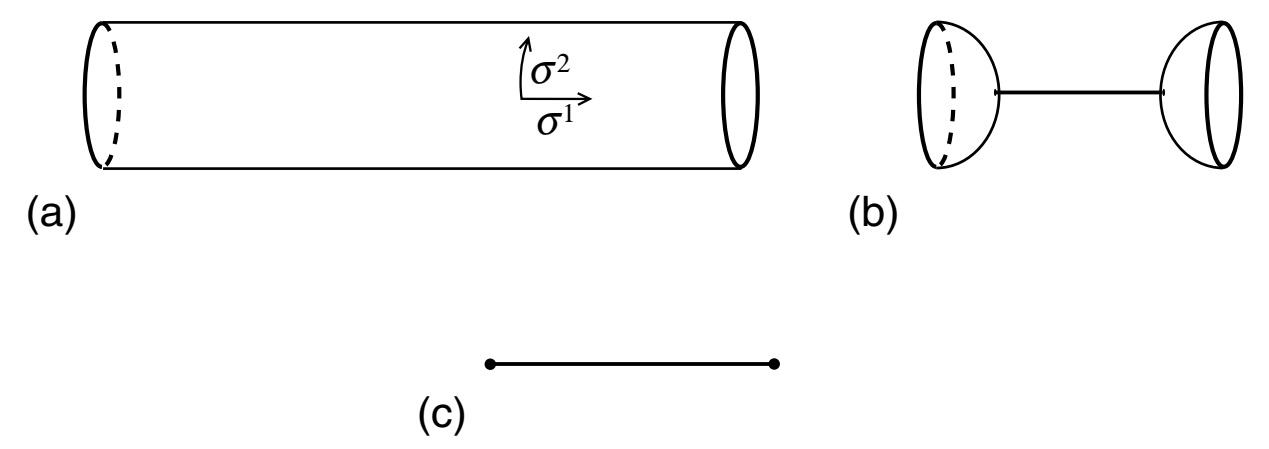
\includegraphics[width=0.8\textwidth,natwidth=951.75,natheight=314.3]{Fig7.1.jpg}\\
		\caption{Fig. 7.1. (a) Cylinder in the limit of small $t$. (b) The amplitude separated into disk tadpole amplitudes and a closed string propagator. (c) Analogous field theory graph. The heavy circles represent the tadpoles.}\label{Fig7.1}
	\end{center}
\end{figure}

它看起来像闭弦从真空中出现,传播了一段距离,又消失在真空中. 为了使其更显然,使用模变换 (7.2.44)
\begin{equation}
	\eta(i t)=t^{-1 / 2} \eta(i / t)
\end{equation}
并将变量改成$s=\pi / t$, 结果是
\begin{equation}
	Z_{C_{2}}=i \frac{V_{26} n^{2}}{2 \pi\left(8 \pi^{2} \alpha^{\prime}\right)^{13}} \int_{0}^{\infty} d s \eta(i s / \pi)^{-24}
\end{equation}
用$1 / t$ 重新标度度规,使得圆柱有闭弦周长 $2 \pi$, 圆柱长度是 $s $. 展开
\begin{equation}
	\begin{aligned}
		\eta(i s / \pi)^{-24} &=\exp (2 s) \prod_{n=1}^{\infty}[1-\exp (-2 n s)]^{-24} \\
		&=\exp (2 s)+24+O(\exp (-2 s))
	\end{aligned}
\end{equation}
这正是用闭弦完备基展开的预期渐近形式. 换句话说,如果我们认为 $\sigma^{2}$ 是世界面时间, $\sigma^{1}$是世界面距离,图(\ref{Fig7.1}a)是一个非常短的开弦圈. 如果我们交换二者的角色,它是一个非常长的闭弦世界线,开端和末端都在边界圆上. 在Euclidean路径积分中,两种描述均可使用,并且在模空间的不同极限下,二者都很有用.\\
真空振幅的领头阶贡献来自闭弦快子. 这是无趣的,它可以通过解析延拓定义
\begin{equation}
	\int_{0}^{\infty} d s \exp (\beta s) \equiv-\frac{1}{\beta}
\end{equation}
第二项来自无质量闭弦态,即使有了延拓也给出形如 $1 / 0$ 的发散. 为了看到这一发散的起源,像图(\ref{Fig7.1}b)那样将过程解离. 正如我们在6.6节看到的,这是在圆盘上有一闭弦顶点算符的非零振幅. 蝌蚪图对应于闭弦消失或出现在真空中. 在动量空间中,无质量传播子正比于 $1 / k^{2} $ . 这里,动量守恒要求从真空中出现的闭弦动量为零,所以传播子发散.\\
在量子场论也有相同类型发散. 考察无质量标量场 $\phi$ 且在Lagrangian中有 $\phi$ 的线性项. 那么就会有只与一个传播子相连的顶点,并且图(\ref{Fig7.1}c)存在. 这一发散是由于中间传播子是
\begin{equation}
	\left.\frac{1}{k^{2}}\right|_{k^{\mu}=0}
\end{equation}
由于传播子极点对应的是传播的时空距离很长,这是长程 (IR) 发散.\\
量子场论中的UV(紫外)发散和IR(红外)发散有着非常不同的起源. UV发散通常标志着理论的失效,在某个短程处需要新物理. IR发散通常意味着我们问出的问题是错误的,或者展开的方式是错误的. 这里也是如此. 在一般微扰论中,我们围绕 $\phi(x)=0$展开或者某个其他场构型展开. 对于作用量
\begin{equation}
	-\frac{1}{g^{2}} \int d^{d} x\left(\frac{1}{2} \partial_{\mu} \phi \partial^{\mu} \phi+g \Lambda \phi\right)
\end{equation}
运动方程
\begin{equation}
	\partial^{2} \phi=g \Lambda
\end{equation}
不允许 $\phi(x)=0$ 作为解. 我们必须围绕 (7.4.8)的一个解展开;而任何解必须是位置相关的. 相应的振幅是没有发散的,即使右边是一微扰 (我们给圆盘引入了合乎的因子 $g$ ), 由于它是奇异微扰,这是正确的. 特别地,正确背景破坏零阶解的某些Poincare对称性.\\
情况在弦论中是相同的. 圆盘蝌蚪图是源
\begin{equation}
	-\Lambda \int d^{26} x(-G)^{1 / 2} e^{-\tilde{\Phi}}
\end{equation}
它是伸缩子和度规的源. 围绕相应场方程的解(不再是常数) 会给出有效的振幅. 细节有一些复杂,将在第9章进一步讨论.\\
附带地,在超弦理论中,如果树图级背景在超对称下不变,那么它通常没有圈修正.\\
极点 (7.4.6) 是我们在树图振幅中遇到了同类发散,对应长时空距离传播的共振. 如果我们在圆柱的每一端加开弦顶点算符,使得它代表开弦一圈振幅,那么从一个边界流向另一个边界的动量 $k^{\mu}$ 一般不为零. 那么大s极限 (7.4.4)会引入因子
\begin{equation}
	\exp \left(-\alpha^{\prime} k^{2} s / 2\right)
\end{equation}
发散变成一个动量极点,它表示开弦散射成闭弦中间态. 因此,正如第3章宣称的,开弦理论必须同时纳入闭弦. 移除UV发散的机制在开弦和闭弦中不同. 在闭弦中是模积分上的有效截断;在开弦,以长时空距离的形式,它重新解释为模空间的危险极限.\\
在 (7.4.1) 中,通过将 $\sigma^{2}$当作时间剪开路径积分,我们将圆柱上的路径积分与开弦频谱关联起来. 它也可通过闭弦获得,这时 $\sigma^{1}$ 是时间. 令 $\sigma^{2}$ 拥有周期$2 \pi$ ,$\sigma^{1}=0, s$处为边界. 闭弦在 $\sigma^{1}=0$ 以某态 $|B\rangle$出现,然后再 $\sigma^{1}=s $又以同样方式消失. 引入测度插入,那么路径积分正比于
\begin{equation}
	\left\langle B\left|c_{0} b_{0} \exp \left[-s\left(L_{0}+\tilde{L}_{0}\right)\right]\right| B\right\rangle
\end{equation}
$\partial_{1} X^{\mu}, c^{1}$和 $b_{12}$在边界上为零决定了态 $|B\rangle$. 以 Hamiltonian形式,它们必须湮灭 $|B\rangle$, 以Laurent系数的形式
\begin{equation}
	\left(\alpha_{n}^{\mu}+\tilde{\alpha}_{-n}^{\mu}\right)|B\rangle=\left(c_{n}+\tilde{c}_{-n}\right)|B\rangle=\left(b_{n}-\tilde{b}_{-n}\right)|B\rangle=0, \quad \text { all } n
\end{equation}
这给出
\begin{equation}
	|B\rangle \propto\left(c_{0}+\tilde{c}_{0}\right) \exp \left[-\sum_{n=1}^{\infty}\left(n^{-1} \alpha_{-n} \cdot \tilde{\alpha}_{-n}+b_{-n} \tilde{c}_{-n}+\tilde{b}_{-n} c_{-n}\right)\right]|0 ; 0\rangle
\end{equation}
将其用于 (7.4.11) 给出 (7.4.3), 还未决定的是 $|B\rangle$ 的归一化. 这个表示在分析 $t \rightarrow 0$的极限以及闭弦极点时候非常有用.\\
通过比较弦论计算与场论计算我们可以决定圆盘蝌蚪 $\Lambda$, 但在下一章,将其作为一个更一般结果的特殊情况进行处理将会更加方便.\\

\centerline{\Large Klein瓶}
来自Klein瓶的真空振幅是
\begin{equation}
	\begin{aligned}
		Z_{K_{2}} &=\int_{0}^{\infty} \frac{d t}{4 t} \operatorname{Tr}_{c}^{\prime}\left\{\Omega \exp \left[-2 \pi t\left(L_{0}+\tilde{L}_{0}\right)\right]\right\} \\
		&=i V_{d} \int_{0}^{\infty} \frac{d t}{4 t}\left(4 \pi^{2} \alpha^{\prime} t\right)^{-d / 2} \sum_{i \in \mathscr{H}_{c}^{\perp}} \Omega_{i} \exp \left[-2 \pi t\left(h_{i}+\tilde{h}_{i}-2\right)\right]
	\end{aligned}
\end{equation}
其中记号来自圆柱(7.4.1). 与定向理论的环面相比,这有一个额外因子 $\frac{1}{2}$ ,它来自投影算符$\frac{1}{2}(1+\Omega) $ . 由于相同原因,在非定向理论中的环面振幅和圆柱振幅均有一个额外因子 $\frac{1}{2}$ . 也可认为这来自额外的规范不变性 $w \rightarrow \bar{w}$. 为了计算26平坦维中的迹,注意$\Omega$ 的的唯一对角元是那些在左移和右移处于相对态,而这些态的贡献是 $\Omega=+1 $ . 这样,迹实际上只取在一边,这与开弦振幅相同,不同的是权重加倍,这是因为左移与右移贡献相同. 结果是
\begin{equation}
	Z_{K_{2}} \rightarrow i V_{26} \int_{0}^{\infty} \frac{d t}{4 t}\left(4 \pi^{2} \alpha^{\prime} t\right)^{-13} \eta(2 i t)^{-24}
\end{equation}
模 $t$ 与圆柱有着相同的取值范围 $0<t<\infty$ ,所以 $t \rightarrow 0$ 发散是相同的. 同样,$1 / 0$极点可以以闭弦极点的形式有一个长程解释. 为了看到这一点,考察区域
\begin{subequations}
\begin{equation}
0 \leq \sigma^{1} \leq 2 \pi, \quad 0 \leq \sigma^{2} \leq 2 \pi t 
\end{equation}
\begin{equation}
0 \leq \sigma^{1} \leq \pi, \quad 0 \leq \sigma^{2} \leq 4 \pi t
\end{equation}		
\end{subequations}
这两个均是基本域,等价关系
\begin{equation}
	w \cong w+2 \pi \cong-\bar{w}+2 \pi i t
\end{equation}
在(7.4.16a)中,左边缘和右边缘周期等价,而上边缘和下边缘在宇称反演后等价,这解释了带有权重$\Omega $的闭弦圈. 对于(7.4.16b), 等价关系 (7.4.17)同时暗示了
\begin{equation}
	w \cong w+4 \pi i t, \quad w+\pi \cong-(\bar{w}+\pi)+2 \pi i t
\end{equation}
由此得出,区域 (7.4.16b)的上边缘和下边缘周期等价. 在左边缘在平移它的一半长度后,通过该边缘的反演与自身等价. 对于右边缘类似:这是十字帽的定义. 因此我们有了图\ref{Fig7.2}a的解释. \\
\begin{figure}
	\begin{center}
		%width=0.8\textwidth,bb=0 0 1256 248
		%1px=0.75pt
		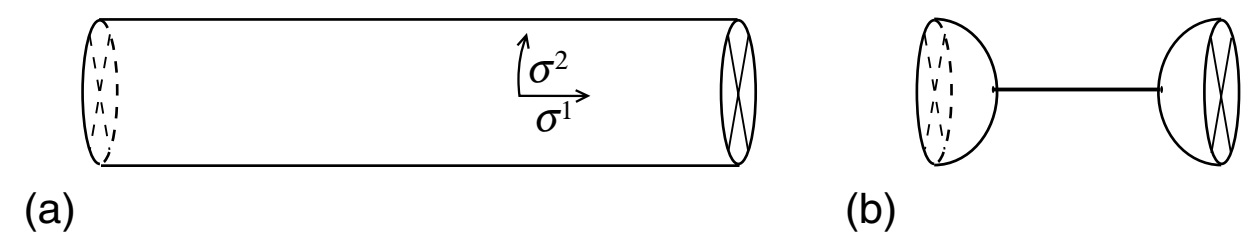
\includegraphics[width=0.8\textwidth,natwidth=879.2,natheight=173.6]{Fig7.2.jpg}\\
		\caption{Fig. 7.2. (a) Klein bottle in the limit of small $t$ as a cylinder capped by crosscaps. (b) The amplitude separated into $R P_{2}$ tadpole amplitudes and a closed string propagator.}\label{Fig7.2}
	\end{center}
\end{figure}

圆柱两端接上十字帽,重新标度$1 / 2 t$, 圆柱底长$2 \pi$,高 $s=\pi / 2 t$. 在模变换后,振幅变成
\begin{equation}
	Z_{K_{2}}=i \frac{2^{26} V_{26}}{4 \pi\left(8 \pi^{2} \alpha^{\prime}\right)^{13}} \int_{0}^{\infty} d s \eta(i s / \pi)^{-24}
\end{equation}

所有关于圆柱的发散的讨论均可用于Klein瓶. 所不同的是蝌蚪图来自于射影平面而非圆盘.\\

\centerline{\Large Möbius带}
对于Möbius带,
\begin{equation}
	Z_{M_{2}}=i V_{d} \int_{0}^{\infty} \frac{d t}{4 t}\left(8 \pi^{2} \alpha^{\prime} t\right)^{-d / 2} \sum_{i \in \mathscr{H}_{0}^{\perp}} \Omega_{i} \exp \left[-2 \pi t\left(h_{i}-1\right)\right]
\end{equation}
它与圆柱上的结果只差 $\Omega$ 以及投影算符的 $\frac{1}{2}$ .在26平坦维中,算符$\Omega$的效应在迹中是:在偶质量能级上有一个额外的$-1$ 再加上对Chan-Paton因子的合理计数. 因此,振子的迹是
\begin{equation}
	\exp (2 \pi t) \prod_{n=1}^{\infty}\left[1-(-1)^{n} \exp (-2 \pi n t)\right]^{-24}=\vartheta_{00}(0,2 i t)^{-12} \eta(2 i t)^{-12}
\end{equation}
对于 $S O(n)$理论, $\frac{1}{2} n(n+1)$ 对称态有$\Omega=+1$,而 $\frac{1}{2} n(n-1)$ 个反对称态有 $\Omega=-1$ ,净贡献为$n$ . 对于$S p(k)$ 理论则相反,给出 $-n$ (在我们的记法中$n=2 k$个 Chan-Paton态). 那么振幅是
\begin{equation}
	Z_{M_{2}}=\pm i n V_{26} \int_{0}^{\infty} \frac{d t}{4 t}\left(8 \pi^{2} \alpha^{\prime} t\right)^{-13} \vartheta_{00}(0,2 i t)^{-12} \eta(2 i t)^{-12}
\end{equation}
通过与Klein瓶相同的构造, Möbius带也可表示为带底的圆柱,这时只有一端是十字帽,如图\ref{Fig7.3}a所示. 

\begin{figure}
	\begin{center}
		%width=0.8\textwidth,bb=0 0 1278 245
		%1px=0.75pt
		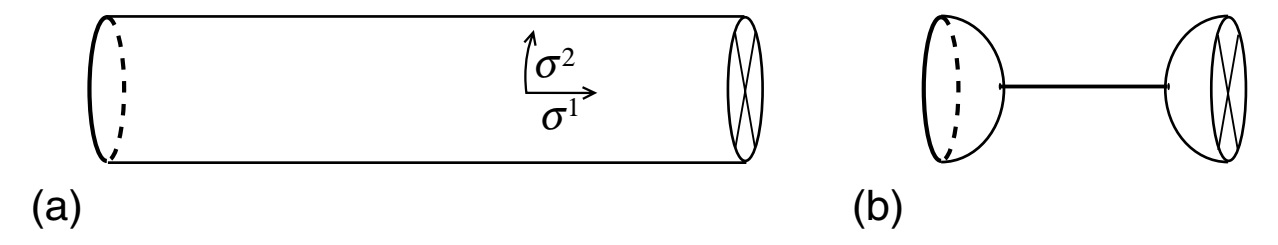
\includegraphics[width=0.8\textwidth,natwidth=894.6,natheight=171.5]{Fig7.3.jpg}\\
		\caption{Fig. 7.3. (a) Möbius in the limit of small $t$ as a cylinder capped by one cross-cap. (b) The amplitude separated into $D_{2}$ and $R P_{2}$ tadpole amplitudes and a closed string propagator.}\label{Fig7.3}
	\end{center}
\end{figure}

圆柱长度现在是$s=\pi / 4 t$. 通过模变换,振幅是
\begin{equation}
Z_{M_{2}}=\pm 2 i n \frac{2^{13} V_{26}}{4 \pi\left(8 \pi^{2} \alpha^{\prime}\right)^{13}} \int_{0}^{\infty} d s \vartheta_{00}(0,2 i s / \pi)^{-12} \eta(2 i s / \pi)^{-12}
\end{equation}
和圆环一样,这也可以写成算符表达式. (7.4.11) 中的一个边界态被替换成了类似的十字帽态 $|C\rangle $ . 这也是 $t \rightarrow 0$ 发散,它对应图\ref{Fig7.3}a的过程,一端来自于圆盘,另一端来自射影平面. 在非定向理论,这三个曲面的发散结合成
\begin{equation}
	i \frac{24 V_{26}}{4 \pi\left(8 \pi^{2} \alpha^{\prime}\right)^{13}}\left(2^{13} \mp n\right)^{2} \int_{0}^{\infty} d s
\end{equation}
即,总的蝌蚪图正比于 $2^{13} \mp n $. 对于规范群 $S O\left(2^{13}\right)=S O(8192)$ 这为零. 来自圆盘的蝌蚪图与来自射影平面的蝌蚪图抵消. 对于玻色弦理论,这或许没什么特殊含义,但在超弦中,对于 $S O(32)$确实有类似的抵消.